
\documentclass[11pt]{article}
\renewcommand{\baselinestretch}{1.05}
\usepackage{amsmath,amsthm,verbatim,amssymb,amsfonts,amscd, graphicx}
\usepackage{graphics}
\topmargin0.0cm
\headheight0.0cm
\headsep0.0cm
\oddsidemargin0.0cm
\textheight23.0cm
\textwidth16.5cm
\footskip1.0cm


\usepackage{graphicx}


\begin{document}



\title{Homework 1 Machine Learning}
\author{Marco Treglia}
\date{}
\maketitle

\section{Principal Component Analisys}
Principal component analysis (PCA) is a mathematical procedure that transforms a number of (possibly) correlated variables into a (smaller) number of uncorrelated variables called principal components. PCA has many applications;

First, compression representing $x(i)$  with lower dimension $y(i)$ were, $x(i)$  is the data set given ${x(i); i = 1, . . . , m}$. and $y(i)$  is the data set after the PCA.

Another standard application is to preprocess a dataset to reduce its dimension before running a supervised learning  algorithm with the $x(i)$s as inputs. Apart from computational benefits, reducing the data’s dimension can also reduce the complexity of the hypothesis class considered and help avoid overfitting.

Lastly, we can also view PCA as a noise reduction algorithm.

\section{Mathematical step}


\subsection{Pre-processing data}
Prior to running PCA per se, typically we first pre-process the data to normalize its mean and variance, as follows:

1. Let $\mu=\frac{1}{m} \sum\limits_{i=1}^m x^{(i)}.$

2. Replace each $x(i)$ with $x(i) - \mu$ .

3. Let $\sigma^2_{j} = \frac{1}{m} \sum\limits_{i} (x^{(i)}_{j})^2$

4. Replace each $x^{(i)}_{j}$ with $\frac{x^{(i)}_{j}}{\sigma^2_{j}}$.

\subsection{Covariance Matrix}
First compute the covariance matrix of the data,  which is a d x d  matrix where each element represents the covariance between two features. The covariance between two features is calculated as follows: :

$$\sigma_{jk} \; =\; \frac{1}{n\; -\; 1}\; \sum_{i=1}^{N}{\left( \left( x_{ij}\; -\; \overline{x}_{j} \right)\left( x_{ik}\; -\; \overline{x}_{k} \right) \right)}$$

where the $\overline{x}$ is the mean vector :

$$\overline{x} = \sum\limits_{k=1}^n{x_{i}} $$



\subsection{Eigenvector and eigenvalue}
From the covariance matrix compute the eigenvectors and eigenvalues. This represent the “core” of a PCA: The eigenvectors (principal components) determine the directions of the new feature space, and the eigenvalues determine their magnitude. In other words, the eigenvalues explain the variance of the data along the new feature axes.

\section{Principal Component Visualization}
For this section i chosed the first four image, loaded with PIL.image, prepocessed for standardize the data then compute the principale component analisys.
\subsection{First and Second Componet}
\begin{center}
 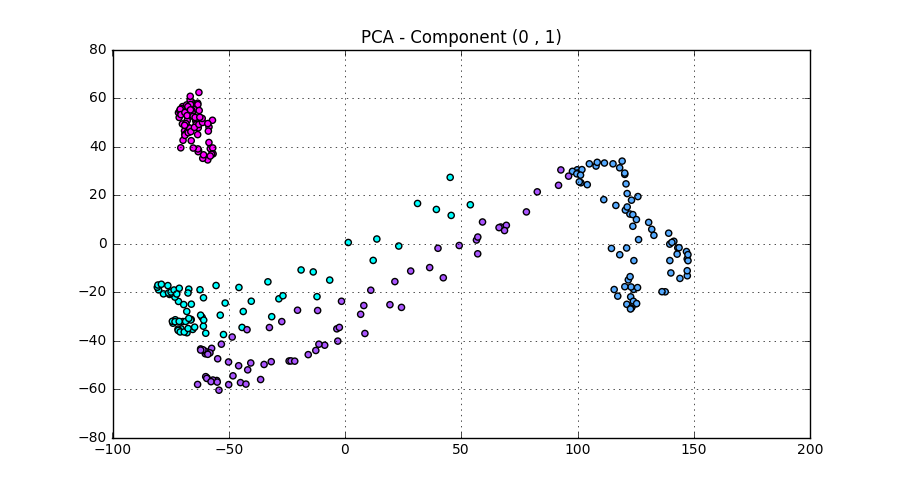
\includegraphics[scale=0.5]{1}
\end{center}

\subsection{Third and Four Componet}
\begin{center}
 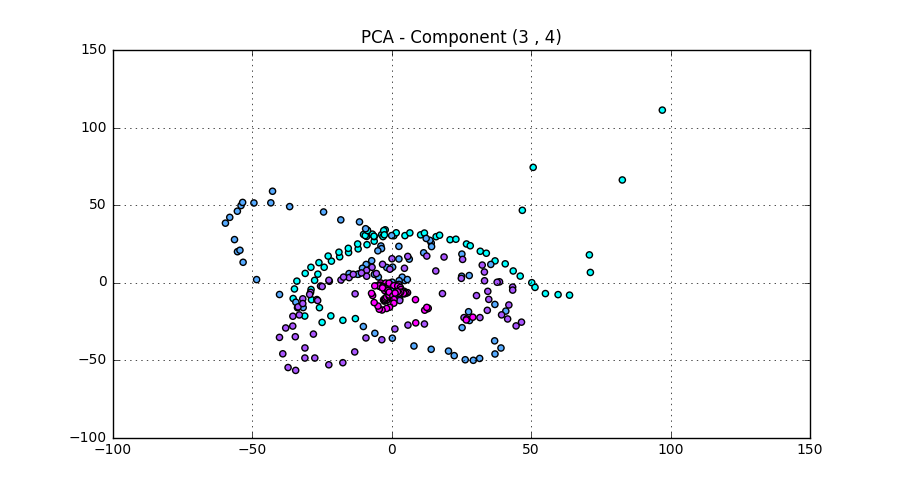
\includegraphics[scale=0.5]{2}
\end{center}

\subsection{Thenth and Eleventh Componet}
\begin{center}
 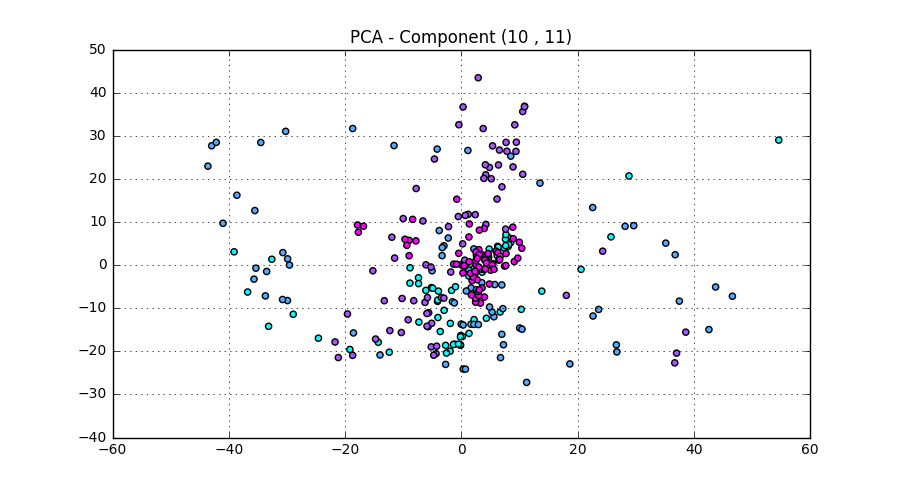
\includegraphics[scale=0.5]{3}
\end{center}



\subsection{Principale component needed}
For determinade the principale component needed for getting the best evaluation of the data , it can be used the explained variance. This tells us how much information (variance) can be attributed to each of the principal components.

\begin{center}
 \begin{tabular}{||c c c||}
  \hline
  Component & Unitary Variance & Cumulative Variance \\ [0.5ex]
  \hline\hline
  1         & 64,77\%          & 64,77 \%            \\
  \hline
  2         & 12,81\%          & 77,58 \%            \\
  \hline
  3         & 10,15\%          & 87,73 \%            \\
  \hline
  4         & 6,81\%           & 94,54 \%            \\
  \hline
  5         & 5,46\%           & 100 \%              \\ [1ex]
  \hline
 \end{tabular}
\end{center}

\begin{center}
 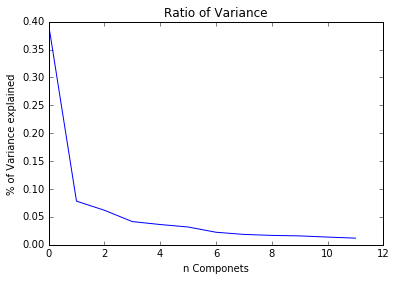
\includegraphics[scale=0.5]{var}
\end{center}

\section{Classification with Naive Bayes}

The Bayesian Classification represents a supervised learning method as well as a statistical method for classification.provides practical learning algorithms and prior knowledge and observed data can be combined.

\subsection{First and Second Component prediction}

\begin{center}
 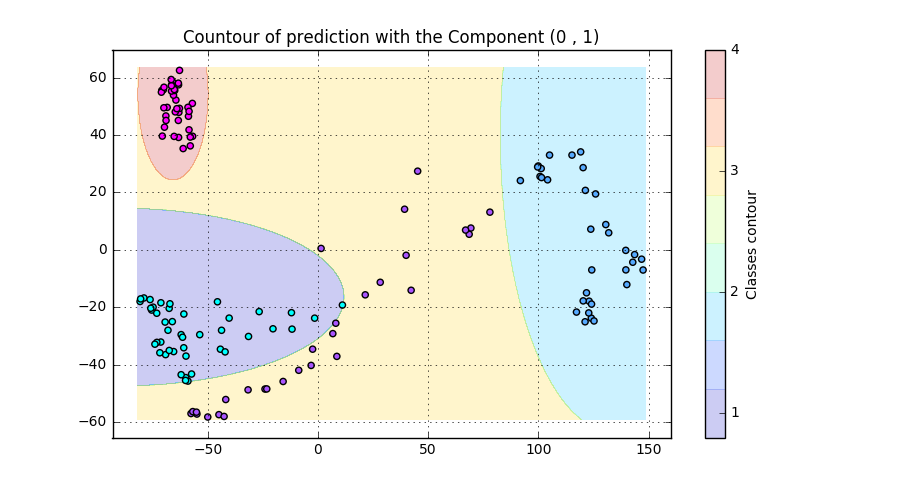
\includegraphics[scale=0.5]{4}
 
 Accuracy of  90.277 \%
\end{center}

\subsection{Third and Four Component prediction}

\begin{center}
 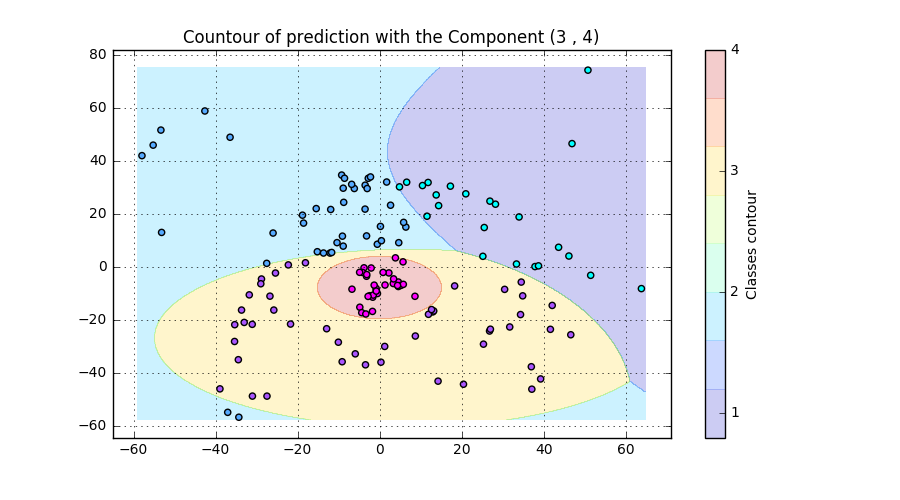
\includegraphics[scale=0.5]{5}
 
 Accuracy of  59.722 \%
\end{center}

\subsection{Thenth and Eleventh Component prediction}

\begin{center}
 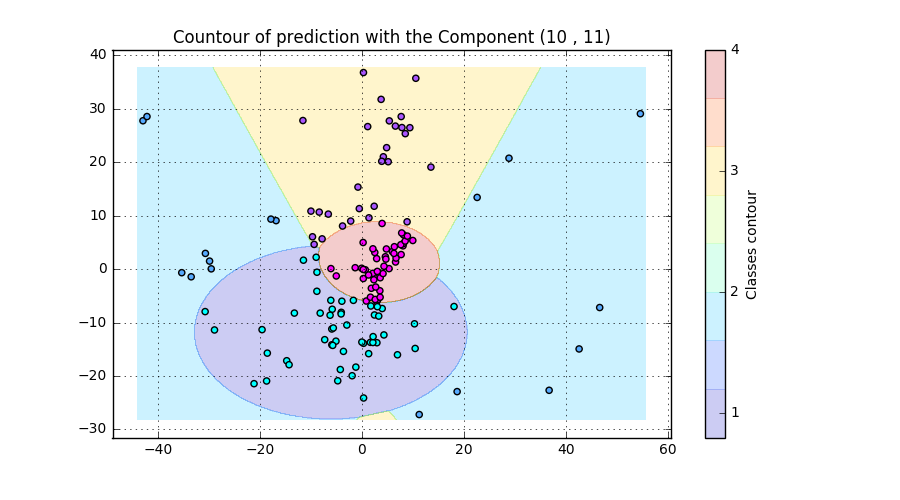
\includegraphics[scale=0.5]{6}
 
 Accuracy of  50.694 \%
\end{center}


\end{document}
